% !TEX root = ../main.tex
\subsection{CEBAF} \label{ssec::cebaf}
    \begin{figure}[b!]
        \centering\frame{
        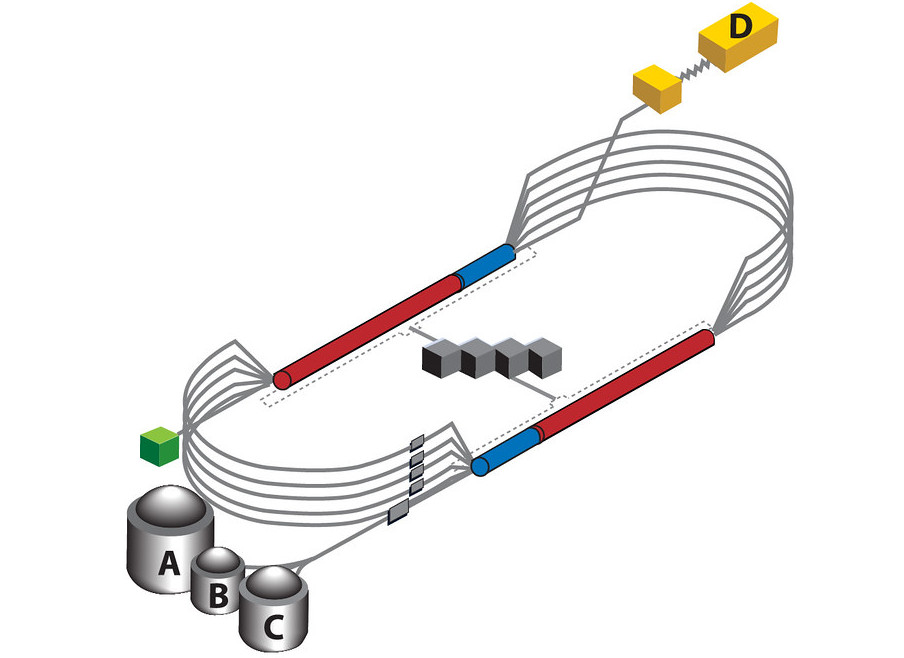
\includegraphics[width=\textwidth]{11experiment/img/10cebaf_diagram.jpg}}
        \caption[CEBAF.]{Simplified representation of CEBAF.
        Source: \hyperlink{https://www.jlab.org/}{jlab.org}.}
        \label{fig::cebaf}
    \end{figure}
    
    CEBAF is a pair of $1.4$-km antiparallel superconducting radio-frequency (RF) linear accelerators (linacs) built 8 meters below the surface.
    Both accelerators are joined by two $180\degree$ arcs, which have a radius of $80$ meters \cite{leemann2001} each.
    A figure detailing the design of CEBAF is available in Figure \ref{fig::cebaf}.

    The recirculating arcs are composed of five separate beamline sections, allowing the beam to cross both linacs up to five times.
    For each linac, the gain in energy of the beam varies between $0.8$ GeV up to $1.2$ GeV, giving it a final energy of about $12$ GeV.
    CEBAF is designed for the experimental study of the structure of mesons, nucleons, and nuclei through the high energy electron beam \cite{rode2010}.
